\subsection{The Native Function}

First, the goal is to write a native function, which performs a matrix-matrix multiplication. The shape has to be suitable for the operation, but it is arbitrary within the limits. It is defined based upon the dimensions m, n and k, as seen in figure \ref{fig:matrix1}, and the matrices A and B computed by the driver.

\begin{figure}[h!] 
	\begin{center}
		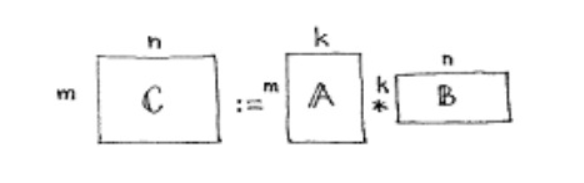
\includegraphics[width=0.9 \textwidth]{fig/matrix1.PNG} 
		\caption{Arbitrary matrix dimensions given in the assignment.}
		\label{fig:matrix1}
	\end{center}
\end{figure}


To create the code for such an operation, the native way is chosen, where the matrix is described using double pointers, i.e. A[i][j]. The choice of function prototypes and driver therefore follows, which is described in the given README file.  \\
The general function prototype used is displayed below:
\begin{lstlisting}[language=C++, caption=Function Prototype]
void matmult_NNN(int m, int n, int k, double ** A, double ** B, double ** C)
\end{lstlisting}

The function prototypes are all declared in the header file ass1\_lib.h. The functions themselves are described in the ass1\_lib.cpp file, where the ass1\_lib.h library is included. \\

The native function takes the integer arguments m, n and k, as well as the double arguments **A, **B and **C. The double arguments are the actual matrices computed, which in the case of matrix A and B are generated within the supplied driver based on the submitted shape parameters. A dynamic memory allocation function is likewise implemented for the three matrices. In the case of C, only the memory is allocated. To perform the matrix-matrix multiplication 3 nested for loops, one for each of the 3 shape parameters, are required. Three loop variables i, j and l are introduced for the matrix leading dimensions m, n and k. The C matrix has the leading dimensions of m and n, C[i][j]. The function is displayed below:

\begin{lstlisting}[language=C++, caption=Function Prototype]
void matmult_nat(int m, int n, int k, double ** A, double ** B, double ** C){
	for(int i = 0; i < m;i++){
		for(int j = 0; j < n;j++){
			C[i][j] = 0;
			for(int l = 0; l < k;l++){
				C[i][j] += A[i][l]*B[l][j];
			}
		}
	}
}
\end{lstlisting}

Notice the += sign, which is caused by the fact, that when the function loops over l for a set (i,j), the multiplications for the different values of l are added together.


\subsection{DGEMM and Comparison}

For comparison reasons, the important subroutine for matrix matrix multiplication DGEMM (Double Precision General Matrix Matrix) from the BLAS library is implemented in our system. The blas.h library is therefore included by using external C. The library function is implemented taking the same arguments as the nat function.

\begin{lstlisting}[language=C++, caption=lib]
void matmult_lib(int m, int n, int k, double ** A, double ** B, double ** C){
  cblas_dgemm(CblasRowMajor, CblasNoTrans, CblasNoTrans, 
  m, n, k, 1.0 , A[0], k, B[0], n, 0.0, C[0], n);
}
\end{lstlisting}

Comparing the two functions clearly display the limits of the native function. Running the two function on the cluster for a few different matrix sizes.


\begin{table}[h!]
\centering
\caption{This table displays the performance (MFlop/s) of the two functions matmult\_nat() and matmult\_lib() with a square matrix size of 512x512 and 2048x2048.}
\label{Table:nat}
\begin{tabular}{|l|l|l|}
\hline m, n, k dimension  & nat() MFlop/s  & lib() MFlop/s \\ \hline
	512 &	529.2 & 20767.1 \\ \hline	
		2048 &	407.2 & 21521.5 \\ \hline	
\end{tabular}
\end{table}



